\documentclass{SchoolBook}

\usepackage{lipsum}
\usepackage{tikz}
\usepackage{amsmath}
\usepackage{multicol}
\usepackage{icomma}
\usepackage{graphicx}
\usepackage{pgfplots}
\pgfplotsset{compat=1.16}

\graphicspath{ {./Images/} }

\tikzset{
  jumpdot/.style={mark=*,solid},
  excl/.append style={jumpdot,fill=white},
  incl/.append style={jumpdot,fill=black},
}

\begin{document}
    \begin{day}{22/04/2021}
        \begin{enumerate}
            \item[1.] Sobre um corpo de massa $ 8 kg $, inicialmente em repouso, age uma força constante $ \vec{F} = 80 N $, na direção do deslocamento.
            Determine o trabalho realizado pela foça nos primeiros 20 segundos de movimento.
            \begin{align*}
                        \tau &= 80 * \Delta S   \\ 
                    \Delta S &= 0,5 * a * 20^2  \\
                          80 &= 8 * a           \\
                \frac{80}{8} &= a               \\
                    10 m/s^2 &= a               \\
                    \Delta S &= 0,5 * 10 * 20^2 \\
                    \Delta S &= 2000 metros
            \end{align*}

            \item[2.] Um ponto material de massa $ 6 kg $ tem velocidade de $ 8 m/s $ quando sobre ele passa a agir uma força de intensidade $ 30 N $ na direção do movimento, durante $ 4 s $. Determine:
            \begin{enumerate}
                \item[a)] o deslocamento durante esses $ 4 s$;
                \begin{align*}
                        \Delta S &= 8 + 0,5 * a * 4^2 \\
                              30 &= 6 * a             \\
                    \frac{30}{6} &= a                 \\
                         5 m/s^2 &= a                 \\
                        \Delta S &= 8 + 0,5 * 5 * 4^2 \\
                        \Delta S &= 169 metros
                \end{align*}
                
                \item[b)] o trabalho realizado nesse deslocamento.
                \begin{align*}
                    \tau &= 30 * 168 \\
                    \tau &= 5040
                \end{align*}
            \end{enumerate}

            \item[3.] Um móvel de massa $ 40 kg $ tem velocidade constante de $ 90 km/h $.
            Num determinado instante entra numa região rugosa onde o coeficiente de atrito é igual a $ 0,2 $. Determine:
            \begin{enumerate}
                \item[a)] o espaço percorrido pelo móvel na região rugosa, até parar;
                \begin{align*}
                             F_{at} &= 0,2 * 40 * 9,8             \\
                             F_{at} &= 78,4 newtons               \\
                               78,4 &= 40 * a                     \\
                    \frac{78,4}{40} &= a                          \\
                         1,96 m/s^2 &= a                          \\
                                0^2 &= 25^2 + 2 * 1,96 * \Delta S \\
                           \Delta S &= 159,43877551 metros
                \end{align*}
                
                \item[b)] o trabalho realizado pela força de atrito.
                \begin{align*}
                    \tau &= 78,4 * 159,43877551 * \cos(180) \\
                    \tau &= 12499,999999984 * -1            \\
                    \tau &= -12499,999999984 joules
                \end{align*}
            \end{enumerate}
        \end{enumerate}
    \end{day}
    
    \begin{day}{26/04/2021}
        \title{3}{Termometria}
        
        Temperatura é uma grandeza física que mede o estado de \textbf{agitação das partíulas} de um corpo, caracterizando o seu estado térmico.
        
        \title{3}{Calor}
        
        É energia térmica \textbf{em trânsito}, entre dois corpos ou sistemas, decorrente apenas da existência de uma diferença de temperatura entre eles.
        
        \title{3}{Escalas Termométricas}
        
        Uma escala termométrica corresponde a um conjunto de valores numéricos, onde cada um desses valores está associado a uma temperatura.
        
        Para a graduação das escalas foram escolhidos, para pontos fixos, dois fenômenos que se reproduzem sempre nas mesmas condições: a fusão do gelo e a ebulição da água, ambas sob pressão normal.
        
        \vspace{3pt}
        \begin{itemize}[nosep]
            \item Primeiro ponto fixo: corresponde à temperatura de fusão do gelo; chamado ponto do gelo;
            \item Segundo ponto fixo: corresponde à temperatura de ebulição da água; chamado ponto de vapor.
        \end{itemize}
        
        \title{3}{Relações entre as escalas}
        
        Supondo que a grandeza termométrica seja a mesma, podemos relacionar as temperaturas assinaladas pelas escalas termométricas da seguinte forma:
        \vspace{6pt}
        
        \begin{tikzpicture}\setmainfont{Latin Modern Roman}
            % Change from white to gray to enable grid
            \draw [very thin, white,step=1] (-8,0) grid (8,-5);
          % \filldraw [fill=black] (0,0) circle [radius=1.5pt];
            
            \coordinate (HTL) at (-3.5,0);
            \coordinate (HTR) at (3.5,0);
            
            \coordinate (HCL) at (-3.5,-2);
            \coordinate (HCR) at (3.5,-2);
            
            \coordinate (HBL) at (-3.5,-5);
            \coordinate (HBR) at (3.5,-5);
            
            \draw (HTL) -- (HTR);
            \draw (HCL) -- (HCR);
            \draw (HBL) -- (HBR);
            
            \coordinate (VLT) at (-2,0);
            \coordinate (VLM) at (-2,-2);
            \coordinate (VLB) at (-2,-5);
            
            \coordinate (VCT) at (0,0);
            \coordinate (VCM) at (0,-2);
            \coordinate (VCB) at (0,-5);
            
            \coordinate (VRT) at (2,0);
            \coordinate (VRM) at (2,-2);
            \coordinate (VRB) at (2,-5);
            
            \draw [|-|,thick] (VLT) -- (VLB);
            \draw [|-|,thick] (VCT) -- (VCB);
            \draw [|-|,thick] (VRT) -- (VRB);
            
            \draw [dashed] (VLT) to[out=0,in=0,distance=-1cm] (VLB);
            \draw [dashed] (VCT) to[out=0,in=0,distance=-1cm] (VCB);
            \draw [dashed] (VRT) to[out=0,in=0,distance=-1cm] (VRB);
            
            \draw [dashed] (VLM) to[out=0,in=0,distance=0.8cm] (VLB);
            \draw [dashed] (VCM) to[out=0,in=0,distance=0.8cm] (VCB);
            \draw [dashed] (VRM) to[out=0,in=0,distance=0.8cm] (VRB);
            
            \node [above,align=center] at (VLT) {Celsius   \\100};
            \node [above,align=center] at (VCT) {Kelvin    \\373};
            \node [above,align=center] at (VRT) {Fahrenheit\\212};
            
            \node [below,align=center] at (VLB) {0  };
            \node [below,align=center] at (VCB) {273};
            \node [below,align=center] at (VRB) {32 };
            
            \node [below left,align=center] at (VLM) {C};
            \node [below left,align=center] at (VCM) {K};
            \node [below left,align=center] at (VRM) {F};
            
            \node [align=right,left] at (HCL) {Temperatura\\qualquer};
        \end{tikzpicture}
        
        $$ \frac{C-0}{100-0} = \frac{K-273}{373-273} = \frac{F-32}{212-32} \Longrightarrow \frac{C}{100} = \frac{K-273}{100} = \frac{F-32}{180} $$
    \end{day}
    
    \begin{day}{27/04/2021}
        \title{3}{ATIVIDADE}
        
        \begin{enumerate}
            \item[1.] A temperatura normal de um corpo humano é 36°C. Qual é essa temperatura expressa nas escalas Fahrenheit e Kelvin?
            \begin{multicols}{2}
                \begin{align*}
                    \frac{36}{\frac{100}{20}} &= \frac{F - 32}{\frac{180}{20}} \\
                                 \frac{36}{5} &= \frac{F - 32}{9}              \\
                             \frac{F - 32}{9} &= \frac{36}{5}                  \\
                             \frac{F - 32}{9} &= 7,2                           \\
                                       F - 32 &= 7,2 * 9                       \\
                                       F - 32 &= 64,8                          \\
                                            F &= 64,8 + 32                     \\
                                            F &= 96,8 ^\circ Fahrenheit
                \end{align*}\\
                \begin{align*}
                    \frac{36}{\frac{100}{20}} &= \frac{K - 273}{\frac{100}{20}} \\
                                 \frac{36}{5} &= \frac{K - 273}{5}              \\
                            \frac{K - 273}{5} &= \frac{36}{5}                   \\
                            \frac{K - 273}{5} &= 7,2                            \\
                                      K - 273 &= 7,2 * 5                        \\
                                            K &= 36 + 273                       \\
                                            K &= 309 Kelvin
                \end{align*}
            \end{multicols}
            
            \item[2.] Transformar 104°F nas escalas Celsius e Kelvin.
            \begin{multicols}{2}
                \begin{align*}
                    \frac{104 - 32}{\frac{180}{20}} &= \frac{C}{\frac{100}{20}} \\
                                 \frac{104 - 32}{9} &= \frac{C}{5}              \\
                                       \frac{72}{9} &= \frac{C}{5}              \\
                                                  8 &= \frac{C}{5}              \\
                                        \frac{C}{5} &= 8                        \\
                                                  C &= 8 * 5                    \\
                                                  C &= 40 ^\circ Celsius
                \end{align*}
                \begin{align*}
                    \frac{104 - 32}{\frac{180}{20}} &= \frac{K - 273}{\frac{100}{20}} \\
                                 \frac{104 - 32}{9} &= \frac{K - 273}{5}              \\
                                       \frac{72}{9} &= \frac{K - 273}{5}              \\
                                                  8 &= \frac{K - 273}{5}              \\
                                  \frac{K - 273}{5} &= 8                              \\
                                            K - 273 &= 8 * 5                          \\
                                            K - 273 &= 40                             \\
                                                  K &= 40 + 273                       \\
                                                  K &= 313 Kelvin
                \end{align*}
            \end{multicols}
            
            \item[3.] Numa das regiões mais frias do mundo, o termômetro indica -76°F. Qual será o valor dessa temperatura na escala ?
            \begin{align*}
                \frac{-76 - 32}{\frac{180}{20}} &= \frac{C}{\frac{100}{20}} \\
                             \frac{-76 - 32}{9} &= \frac{C}{5}              \\
                                 \frac{-108}{9} &= \frac{C}{5}              \\
                                            -12 &= \frac{C}{5}              \\
                                    \frac{C}{5} &= -12                      \\
                                              C &= -12 * 5                  \\
                                              C &= -60 ^\circ Celsius
            \end{align*}
            
            \item[4.] Ao medir a temperatura de um gás, verificou-se que a leitura era a mesma, tanto na escala Celsius como na Fahrenheit. Qual era essa temperatura?
            \begin{align*}
                \frac{T - 32}{\frac{180}{20}} &= \frac{T}{\frac{100}{20}} \\
                             \frac{T - 32}{9} &= \frac{T}{5}              \\
                                 (T - 32) * 5 &= 9T                       \\
                                     5T - 160 &= 9T                       \\
                                      5T - 9T &= 160                      \\
                                          -4T &= 160                      \\
                                            T &= \frac{160}{-4}           \\
                                            T &= -40^\circ
            \end{align*}
        \end{enumerate}
    \end{day}
    
    \begin{day}{Diego Garcia Perez Biguette, 3º FD --- 03/05/2021}
        \title{3}{Atividades Avaliativas}
        
        Transforme:
        \begin{enumerate}
            \item[a)] 305°F em graus Celsius e Kelvin
            \response{Em:\\
                \quad Celsius: 151,67 °C \\
                \quad Kelvin: 424,67 K
            }
            
            \begin{multicols}{2}
                \begin{align*}
                    \frac{305-32}{\frac{180}{20}} &= \frac{C}{\frac{100}{20}} \\
                                    \frac{273}{9} &= \frac{C}{5} \\
                                     30,333333333 &= \frac{C}{5} \\
                                      \frac{C}{5} &= 30,333333333 \\
                                                C &= 30,333333333 * 5 \\
                                                C &= 151,666666667^\circ Celsius
                \end{align*} \\
                \begin{align*}
                    \frac{305-32}{\frac{180}{20}} &= \frac{K-273}{\frac{100}{20}} \\
                                    \frac{273}{9} &= \frac{K-273}{5} \\
                                     30,333333333 &= \frac{K-273}{5} \\
                                  \frac{K-273}{5} &= 30,333333333 \\
                                            K-273 &= 30,333333333 * 5 \\
                                            K-273 &= 151,666666665 \\
                                                K &= 151,666666665 + 273 \\
                                                K &= 424,666666665 Kelvin
                \end{align*}
            \end{multicols}
            
            \item[b)] 100°C em graus Fahrenheit e Kelvin
            \response{Em:\\
                \quad Fahrenheit: 212 °F \\
                \quad Kelvin: 293 K
            }
            
            \begin{multicols}{2}
                \begin{align*}
                    \frac{100}{\frac{100}{20}} &= \frac{F-32}{\frac{180}{20}} \\
                                 \frac{100}{5} &= \frac{F-32}{9} \\
                                            20 &= \frac{F-32}{9} \\
                                \frac{F-32}{9} &= 20 \\
                                          F-32 &= 20 * 9 \\
                                          F-32 &= 180 \\
                                             F &= 180 + 32 \\
                                             F &= 212^\circ Fahrenheit
                \end{align*} \\
                \begin{align*}
                    \frac{100}{\frac{100}{20}} &= \frac{K-273}{\frac{100}{20}} \\
                                 \frac{100}{5} &= \frac{K-273}{5} \\
                                            20 &= \frac{K-273}{5} \\
                               \frac{K-273}{5} &= 20 \\
                                         K-273 &= 20 \\
                                             K &= 20 + 273 \\
                                             K &= 293 Kelvin
                \end{align*}
            \end{multicols}
            
            \item[c)] 293K  em graus Celsius e Fahrenheit
            \response{Em: \\
                Celsius: 20 °C \\
                Fahrenheit: 68 °F
            }
            
            \begin{multicols}{2}
                \begin{align*}
                    \frac{293-273}{\frac{100}{20}} &= \frac{C}{\frac{100}{20}} \\
                                 \frac{293-273}{5} &= \frac{C}{5} \\
                                      \frac{20}{5} &= \frac{C}{5} \\
                                                 4 &= \frac{C}{5} \\
                                       \frac{C}{5} &= 4 \\
                                                 C &= 4 * 5 \\
                                                 C &= 20^\circ Celsius
                \end{align*} \\
                \begin{align*}
                    \frac{293-273}{\frac{100}{20}} &= \frac{F-32}{\frac{180}{20}} \\
                                 \frac{293-273}{5} &= \frac{F-32}{9} \\
                                      \frac{20}{5} &= \frac{F-32}{9} \\
                                                 4 &= \frac{F-32}{9} \\
                                    \frac{F-32}{9} &= 4 \\
                                              F-32 &= 4 * 9 \\
                                              F-32 &= 36 \\
                                                 F &= 36 + 32 \\
                                                 F &= 68^\circ Fahrenheit
                \end{align*}
            \end{multicols}
        \end{enumerate}
    \end{day}
    
    \begin{day}{04/05/2021}
        \title{3}{Dilatação Térmica}
        
        A esperiência mostra que os sólidos, ao sofrerem um aquecimento, se dilatam e, ao serem resfriados, se contraem.
        
        A dilatação ou a contração ocorrem em 3 dimensões: \textbf{comprimento, largura e espessura}.
        
        A essa variações nas dimensões de um sólido causada pelo aquecimento ou resfriamento denominamos \emph{dilatação térmica}. 
        
        \title{3}{Dilatação Linear}
        
        É aquela em que predomina a variação \textbf{em uma única dimensão}, ou seja, o comprimento.
        
        \begin{center}
            \includegraphics[width=8cm]{Física_04-05-2021}
        \end{center}
        
        Exemplos: dilatação em fios, cabos e barras.
        
        $$ \Delta L = L_i * \alpha * ( T_F - T_i ) $$
        
        \vspace{6pt}
        \begin{tabular}{ r c l }
            $ \Delta L $ &=& Variação de comprimento;         \\
                 $ L_i $ &=& Comprimento inicial;             \\
              $ \alpha $ &=& Coeficiente de Dilatação Linear; \\
                 $ T_F $ &=& Temperatura Final;               \\
                 $ T_i $ &=& Temperatura Inicial
        \end{tabular}
        
        \vspace{6pt}
        
        O comprimento de um fio de alumínio é de 40m a 20°C. Sabendo-se que o fio é aquecido até 60°C e que o coeficiente de dilatação térmica linear do alumínio é de $24 * 10^{-6\circ} C^{-1}$, determinar:
        
        \begin{enumerate}
            \item[a)] a dilatação do fio;
            \response{A dilatação foi de 3,84 centímetros}
            \begin{align*}
                \Delta L &= 40 * (24 * 10^{-6}) * (60 - 20) \\
                \Delta L &= 40 * 0,000024 * 40              \\
                \Delta L &= 0,0384\;m                       \\
                \Delta L &= 3,84\;cm            
            \end{align*}
            
            \item[b)] o comprimento final do fio;
            \response{O comprimento final do fio foi de 40,0384 metros}
            \begin{align*}
                L_F &= L_i + \Delta L \\
                40,0384\;m &= 40 + 0,0384
            \end{align*}
        \end{enumerate}
        
        Uma barra de ferro tem comprimento 10m a 0°C. Sabendo que o coeficiente de dilatação linear do ferro é igual a $12 * 10^{-6\circ}C^{-1}$, calcule:
        
        \begin{enumerate}
            \item[a)] o comprimento final da barra a 20°C;
            \response{O comprimento final da barra é de 10,0024 metros}
            \begin{multicols}{2}
                \begin{align*}
                    \Delta L &= 10 * (12 * 10^{-6}) * (20 - 0) \\
                    \Delta L &= 10 * 0,000012 * 20             \\
                    \Delta L &= 0,0024\;m                       
                \end{align*}
                
                \begin{align*}
                     L_F &= L_i + \Delta L \\
                     L_F &= 10 + 0,0024    \\
                     L_F &= 10,0024\;m
                \end{align*}
            \end{multicols}
            
            \item[b)] o comprimento final da barra a -30°C.
            \response{O comprimento final da barra é de 9,994 metros}
            \vspace{-24pt}
            \begin{multicols}{2}
                \begin{align*}
                    \Delta L &= 10 * (12 * 10^{-6}) * -(20 - (-30)) \\
                    \Delta L &= 10 * (12 * 10^{-6}) * -50           \\
                    \Delta L &= 10 * 0,000012 * -50                 \\
                    \Delta L &= -0,006\;m                           \\
                \end{align*}
                
                \begin{align*}
                     L_F &= L_i + \Delta L \\
                     L_F &= 10 + (-0,006)  \\
                     L_F &= 9,994\;m
                \end{align*}
            \end{multicols}
        \end{enumerate}
        
        Uma barra de alumínio passando de 15°C a 100°C alonga-se 1,224mm. Calcule o comprimento inicial dessa barra. Dado: $\alpha_{Al} = 24 * 10^{-6\circ}C^{-1}$.
        \response{O comprimento inicial dessa barra era de 600mm}
        \begin{align*}
                    1,224 &= L_i * (24 * 10^{-6}) * (100 - 15) \\
                    1,224 &= L_i * 0,000024 * 85               \\
                    1,224 &= L_i * 0,00204                     \\
            L_i * 0,00204 &= 1,224                             \\
                      L_i &= \frac{1,224}{0,00204}             \\
                      L_i &= 600\;mm
        \end{align*}
        
        A que temperatura deve encontrar-se uma trena de aço para que seu comprimento seja 0,5mm maior do que o comprimento de 2000 mm que ela possui à temperatura de 0°C? O coeficiente de dilatação linear do aço vale $1,0 * 10^{-5\circ}C^{-1}$.
        \response{A temperatura deve ser de 25°C}
        \begin{align*}
                         0,5 &= 2000 * (1,0 * 10^{-5}) * (T_F - 0) \\
                         0,5 &= 2000 * 0,00001 * (T_F - 0)         \\
                         0,5 &= 0,02 * (T_F - 0)                   \\
            0,02 * (T_F - 0) &= 0,5                                \\
                   (T_F - 0) &= \frac{0,5}{0,02}                   \\
                     T_F - 0 &= 25                                 \\
                         T_F &= 25 + 0                             \\
                         T_F &= 25^\circ C
        \end{align*}
    \end{day}
    
    \begin{day}{10/05/2021}
        \title{3}{Dilatação Superficial}
        
        É aquela em que predomina a variação em duas dimensões, ou seja, a variação da área.
        
        Consideremos uma placa de área inicial $S_i$, a temperatura inicial $T_i$. Aumentando a temperatura da placa para $T_f$, sua área passa para $S_f$.
        
        $$ \Delta S = S_i * \beta * (T_f - T_i) $$
        $$ \beta = 2\alpha $$
        
        \vspace{6pt}
        \begin{tabular}{ r c l }
            $ \Delta S $ &=& Variação de área;                     \\
                 $ S_i $ &=& Área inicial;                         \\
               $ \beta $ &=& Coeficiente de Dilatação Superficial; \\
                 $ T_f $ &=& Temperatura Final;                    \\
                 $ T_i $ &=& Temperatura Inicial
        \end{tabular}
        \vspace{6pt}
        
        \title{3}{Atividades}
        
        \begin{enumerate}
            \item[1.] Uma placa retângular de alumínio tem 10cm de largura e 40cm de comprimento, à temperatura de 20°C. Essa placa é colocada num ambiente cuja temperatura é de 50°C. Sabendo-se que $\beta_{Al} = 46 * 10^{-6\circ}C^{-1}$, calcular:
            
            \begin{enumerate}
                \item[a)] a dilatação superficial da placa;
                \begin{align*}
                    \Delta S &= (10 * 40) * (46 * 10^{-6}) * (50 - 20) \\
                    \Delta S &= 400 * 0,000046 * 30                    \\
                    \Delta S &= 400 * 0,000046 * 30                    \\
                    \Delta S &= 0,552\;cm^2
                \end{align*}
                
                \item[b)] a área da placa nesse ambiente.
                \begin{align*}
                    S_f &= 400 + 0,552   \\
                    S_f &= 400,552\;cm^2
                \end{align*}    
            \end{enumerate}
            
            \item[2.] Uma placa retangular de alumínio tem área de 40cm² a 0°C. Sabendo que o coeficiente de dilatação superficial do elumínio é $48 * 10^{-6\circ}C^{-1}$, calcule:
            
            \begin{enumerate}
                \item[a)] a área final da placa a 50°C;
                \begin{align*}
                         S_f &= 40 + \Delta S                \\[3pt]
                    \Delta S &= 40 * (48*10^{-6}) * (50 - 0) \\
                    \Delta S &= 40 * 0,000048 * 50           \\
                    \Delta S &= 0,096\;cm^2                  \\[3pt]
                         S_f &= 40 + 0,096                   \\
                         S_f &= 40,096\;cm^2
                \end{align*}
                
                \item[b)] a área final da placa a -20°C.
                \begin{align*}
                         S_f &= 40 + \Delta S             \\[3pt]
                    \Delta S &= 40 * 0,000048 * (-20 - 0) \\
                    \Delta S &= 40 * 0,000048 * -20       \\
                    \Delta S &= -0,0384\;cm^2             \\[3pt]
                         S_f &= 40 + (-0,0384)            \\
                         S_f &= 39,9616\;cm^2
                \end{align*}
            \end{enumerate}
        \end{enumerate}
    \end{day}
    
    \begin{day}{11/05/2021}
        \begin{enumerate}
            \item[3.] Uma chapa tem área de 2 m² a 0°C. Aquecendo-a até 80°C, sua área aumenta de 0,4 cm². Calcule o coeficiente de dilatação supercicial do material que constitui a placa.
            \begin{align*}
                              0,4 &= 200 * \beta * (80 - 0)  \\
                              0,4 &= 200 * \beta * 80        \\
                 200 * \beta * 80 &= 0,4                     \\
                    \beta * 16000 &= 0,4                     \\
                            \beta &= \frac{0,4}{16000}       \\
                            \beta &= 0,000025                \\
                            \beta &= 25 * 10^{-6\;\circ}C^{-1}
            \end{align*}
            
            \item[4.] Um círculo de aço homogêneo, de raio 10 cm e coeficiente dilatação linear $1,2 * 10^{-5\;\circ}C^{-1}$, tem sua temperatura alterada de 10°C para 110°C. Calcule a \textbf{dilatação superficial} sofrida pelo círculo nessa variação de temperatura. Adote $\pi = 3,14$.
            \begin{align*}
                \Delta S &= S_i * 2 * \alpha * (T_f - T_i)         \\[3pt]
                \Delta S &= S_i * 2 * (1,2 * 10^{-5}) * (110 - 10) \\[3pt]
                     S_i &= \pi * r^2                              \\
                     S_i &= 3,14 * 10^2 = 3,14 * 100               \\
                     S_i &= 314                                    \\[3pt]
                \Delta S &= 314 * 2 * (1,2 * 10^{-5}) * (110 - 10) \\
                \Delta S &= 314 * 2 * 0,000012 * 100               \\
                \Delta S &= 0,7536\;cm^2
            \end{align*}
        \end{enumerate}
    \end{day}
    
    \begin{day}{17/05/2021}
        \title{2}{Calorimeria}
        \title{3}{Unidades de Quantidade de Calor}
        
        Antes mesmo que o calor fosse reconhecido como forma de energia, as medidas de quantidade de calor eram feitas através das variações de temperatura que os corpos sofriam quando se lhes fornecia energia sob forma de calor.
        
        Assim, estabeleceu-se como \emph{unidade de quantidade de calor} a caloria (Cal).
        
        No sistema internacional de unidades (SI), a unidade de quantidade de calor é o Joule (J).
        
        $$ 1\;Cal = 4,186\;Joule $$
        
         Podemos utilizar também um múltiplo de caloria chamado quilo-caloria.
         
         $$ 1\;Kcal = 1000\;Cal $$
         
         \title{3}{Calor Sensível e Calor Latente}
         
         Um corpo, ao receber ou ceder calor, pode sofrer dois efeitos diferentes: \emph{variação de temperatura} ou \emph{mudança de fase}.
         
         A quantidade de calor recebida ou cedida por um corpo, ao sofrer uma \textbf{variação de temperatura} sem que haja mudança de fase, é denominado \textbf{calor sensível}.
         
         Se o corpo sofrer apenas uma \textbf{mudança de fase} sem haver variação de temperatura, o calor é chamado \textbf{latente}.
         
         \title{3}{Calor Específico}
         
         A experiência mostra que cada substância necessita de uma quantidade de calor diferente para que 1 grama dessa substância sofra variação de temperatura de 1 celsius.
         
         Essa quantidade é uma característica de cada substância é denominada \textbf{calor específico}, representado pela letra \textbf{c}.
         
         \title{3}{Capacidade Térmica de um Corpo}
         
         É o quociente entre a quantidade de calor ($Q$) recebido ou cedido por um corpo e a correspondente variação de temperatura ($\Delta t$).
         
         $$ C = \frac{Q}{\Delta t} $$
         \begin{center}
            ou
         \end{center}
         $$ C = m * c $$
         A unidade de capacidade térmica é $cal/^\circ C$
         
    \end{day}
    
    \begin{day}{18/05/2021}
        \title{4}{Equação Fundamental da Calorimetria}
        
        $$ Q = m * c * (T_f - T_i) $$
        \begin{center}
            ou
        \end{center}
        $$ Q = m * c * \Delta t $$
        
        \vspace{6pt}
        \begin{tabular}{ r c l }
                   $ Q $ &=& Quantidade de calor;       \\
                   $ m $ &=& Corpo de massa (em grama); \\
                   $ c $ &=& Calor específico;          \\
                 $ T_F $ &=& Temperatura Final;         \\
                 $ T_i $ &=& Temperatura Inicial;       \\
            $ \Delta t $ &=& Diferença de Temperatura 
        \end{tabular}
        \vspace{6pt}
        
        \title{3}{Atividades}
        
        \begin{enumerate}
            \item[1.] Um bloco de ferro com massa de 600 gramas está a uma temperatura de 20°C. O calor específico do ferro é igual a $ 0,114\;cal/g\;^\circ C $.
            \begin{enumerate}
                \item[a)] Qual a quantidade de calor que o bloco deve receber para que sua temperatura passe de 20°C a 50°C?
                \begin{align*}
                    Q &= m * c * (T_f - T_i)     \\
                    Q &= 600 * 0,114 * (50 - 20) \\
                    Q &= 600 * 0,114 * 30        \\
                    Q &= 68,4 * 30               \\
                    Q &= 2052\;cal
                \end{align*}
                
                \item[b)] Qual a quantidade de calor que o bloco deve ceder para que sua temperatura varie de 20°C a -5°C?
                \begin{align*}
                    Q &= m * c * (T_f - T_i)       \\
                    Q &= 600 * 0,114 * ((-5) - 20) \\
                    Q &= 600 * 0,114 * -25         \\
                    Q &= 68,4 * -25                \\
                    Q &= -1710\;cal
                \end{align*}
                
            \end{enumerate}
            
            \item[2.] Sabendo que 1 cal é igual a 4,18 joule:
            \begin{enumerate}
                \item[a)] Tansforme 20 Kcal em Joules.
                \begin{align*}
                    j_{oule} &= 4,186 * cal   \\
                    j_{oule} &= 4,186 * 20000 \\
                    j_{oule} &= 83720\;joules 
                \end{align*}
                
                \item[b)] Transforme 8000 J em Calorias.
                \begin{align*}
                    cal &= \frac{j_{oule}}{4,186} \\
                    cal &= \frac{8000}{4,186}     \\
                    cal &= 1911,13\;cal
                \end{align*}
                
                \item[c)] Um bloco de cobre com 200 grama sofre um aquecimento de 25°C para 70°C. O calor específico do cobre é igual a $ 0,093\;cal/g\;^\circ C $.
                \begin{enumerate}
                    \item[I.] Qual a quantidade de calor recebida pelo bloco?
                    \begin{align*}
                        Q &= 200 * 0,093 * (70 - 25) \\
                        Q &= 200 * 0,093 * 45        \\
                        Q &= 18,6 * 45               \\
                        Q &= 837\;cal
                    \end{align*}
                    
                    \item[II.] Determine a capacidade térmica do bloco.
                    \begin{align*}
                        C &= m * c               \\
                        C &= 200 * 0,093         \\
                        C &= 18,6\;cal/^\circ\;C \\[6pt]
                        C &= \frac{Q}{\Delta t}  \\
                        C &= \frac{837}{70 - 25} \\
                        C &= \frac{837}{45}      \\
                        C &= 18,6\;cal
                    \end{align*}
                \end{enumerate}
            \end{enumerate}
        \end{enumerate}
    \end{day}
    
    \begin{day}{24/05/2021}
        \begin{enumerate}
            \item[3.] Determine quantas calorias perderá 1kg de água para que sua temperatura varie de 60°C para 10°C. O calor específico da água é igual a $ 1\;cal/g^\circ\;C $.
            \begin{align*}
                Q &= m * c * (T_f - T_i)    \\
                Q &= 1000 * 1 * (10 - 60)   \\
                Q &= 1000 * -50             \\
                Q &= -50000\;cal = -50\;Kcal
            \end{align*}
            
            \item[4.] Sabendo que o calor específico do ferro é de aproximadamente $ 0,1\;cal/g^\circ\;C $, calcule a quantidade de calor para elevar 15°C a temperatura de um pedaço de 80g desse material.
            \begin{align*}
                Q &= 80 * 0,1 * \Big((T_i + 15) - T_i\Big)  & Q &= 80 * 0,1 * 15 \\
                Q &= 8 * \Big((T_i + 15) - T_i\Big)         & Q &= 120\;cal      \\
                Q &= \Big(8 * (T_i + 15)\Big) - (8 * T_i)   \\
                Q &= \Big((8 * T_i) + (8 * 15)\Big) - 8 T_i \\
                Q &= 8T_i + 120 - 8T_i                      \\
                Q &= (8T_i - 8T_i) + 120                    \\
                Q &= 120\;cal
            \end{align*}
            
            \item[5.] Um corpo de massa igual a 1 kg recebeu 10000 cal e sua temperatura passou de 50°C para 100°C. Qual o calor específico desse corpo?
            \begin{align*}
                     10000 &= 1000 * c * (100 - 50) \\
                     10000 &= 1000 * c * 50         \\
                     10000 &= 50000 * c             \\
                 50000 * c &= 10000                 \\
                         c &= \frac{10000}{50000}   \\
                         c &= 0,2\;cal/g^\circ\;C
            \end{align*}
        \end{enumerate}
    \end{day}
    
    \begin{day}{25/05/2021}
        \begin{enumerate}
            \item[6.] O calor específico do ferro é igual a $ 0,110\;cal/g^\circ\;C $. Determine a temperatura final de uma massa de 400 grama de ferro á temperatura de 20°C, após ter cedido 500 cal.
            \begin{align*}
                -500 &= 400 * 0,110 * (T_f - 20) \\
                -500 &= 44 * (T_f - 20) \\
                -500 &= (44 T_f) - (44 * 20) \\
                -500 &= 44 T_f - 880 \\
                44 T_f - 880 &= -500 \\
                44 T_f &= -500 + 880 \\
                44 T_f &= 380 \\
                T_f &= \frac{380}{44} \\
                T_f &= 8,636363636^\circ\;C
            \end{align*}
            
            \item[7.] O gráfico representa o aquecimento de 100 grama de uma substância.
            
            \begin{center}
                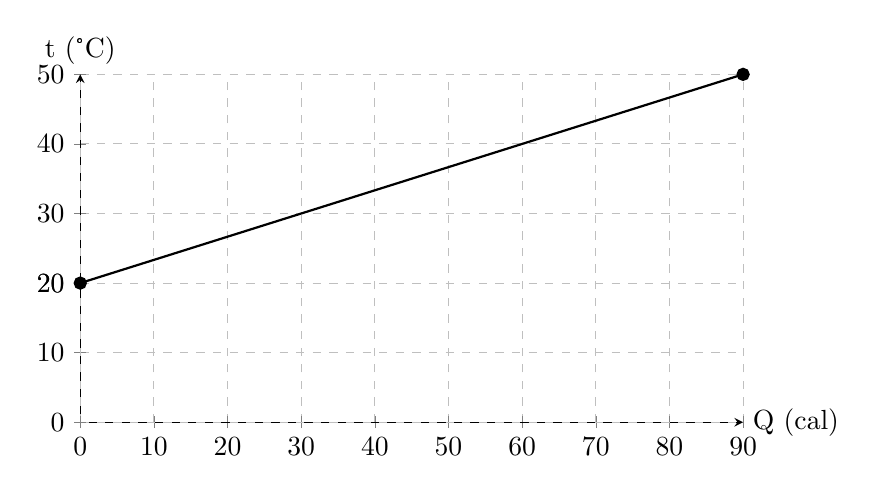
\begin{tikzpicture}
                    \begin{axis}[
                        grid, grid style=dashed,
                        xlabel={Q (cal)},
                        ylabel={t (°C)},
                        xtick={0,10,20,30,40,50,60,70,80,90},
                        ytick={0,10,20,20,30,40,50},
                        ymin=0, ymax=50,
                        xmin=0, xmax=90,
                        width=10cm,
                        height=6cm,
                        ymajorgrids,
                        xmajorgrids,
                        axis lines=middle,
                        extra x ticks={0},
                        extra y ticks={0},
                        x label style={right},
                        y label style={above},
                        %axis on top
                    ]
                        \addplot[
                            color=black,
                            jumpdot,
                            thick, 
                        ] coordinates {(0,20)(90,50)};
                    \end{axis}
                \end{tikzpicture}
            \end{center}
            \begin{enumerate}
                \item[a)] qual o calor específico da substância?
                \begin{align*}
                    90 &= 100 * c * (50 - 20) \\
                    90 &= 100 * c * 30 \\
                    90 &= 3000c \\
                    3000c &= 90 \\
                    c &= \frac{90}{3000} \\
                    c &= 0,03\;cal/g^\circ\;C
                \end{align*}
                
                \item[b)] qual a capacidade térmica da substância?
                \begin{align*}
                    C &= m * c \\
                    C &= 100 * 0,03 \\
                    C &= 3\;cal/^\circ\;C
                \end{align*}
            \end{enumerate}
        \end{enumerate}
        
        \title{3}{Princípio da Igualdade das Trocas de Calor}
        
        Quando dois ou mais corpos com temperaturas diferentes são colocados próximos um do outro ou em contato, eles trocam calor entre si até atingir o equilíbrio térmico.
        
        Se o sistema não trocar energia com o ambiente, isto é, se for termicamente isolado.
        
        Note que a quantidade de calor cedida por A é igual, em valor absoluto, à quantidade de calor recebida por B.
        
        Se tivermos $n$ corpos, teremos:
        $$ Q_1 + Q_2 + Q_3 + \dots + Q_n = 0 $$
        
        Uma xicara de 50g está a 34°C, coloca-se nela 250g de água a 100°C. Verifica-se que no equilíbrio térmico a temperatura é de 94°C, adimitindo que só haja troca de calor entre xícara e a água. Determinar o calor específico da xicara dado: $C_{agua} = 1\;cal/g^\circ\;C$.
        \begin{center}
            \vspace{6pt}
            \begin{tabular}{|c|c|c|c|c|}\hline
                       & m   & c & $T_f$ & $T_i$ \\\hline
                Xícara & 50  & c & 94    & 34    \\\hline
                Água   & 250 & 1 & 94    & 100   \\\hline
            \end{tabular}
        \end{center}
    \end{day}
    
    \begin{day}{31/05/2021}
        \begin{align*}
            (m_{xicara} * c_{xicara} * \Delta T_{xicara}) + (m_{agua} * c_{agua} * \Delta T_{agua}) &= 0 \\
            \Big(50 * c * (94 - 34)\Big) + \Big(250 * 1 * (94 - 100)\Big) &= 0 \\
            (50 * c * 60) + (250 * 1 * -6) &= 0 \\
            3000c + −1500 &= 0 \\
            3000c &= 0 + 1500 \\
            3000c &= 1500 \\
            c &= \frac{1500}{3000} \\
            c &= 0,5\;cal/g^\circ\;C
        \end{align*}
        
        Um calorímetro de capacidade térmica $8\;cal/^\circ\;C$ contém 120 g de água a 15°C. Um corpo de massa $x$ gramas e temperatura 60°C é colocado no interior do calorímetro. Sabendo-se que o calor específico do corpo é de $0,22\;cal/g^\circ\;C$ e que a temperatura de equilíbrio térmico é de 21,6°C , calcular $x$.
        
        \begin{center}
            \vspace{6pt}
            \begin{tabular}{|c|c|c|c|c|}\hline
                            & m   & c    & $T_f$ & $T_i$ \\\hline
                Calorímetro & \multicolumn{2}{|c|}{8} & 21,6  & 15    \\\hline
                Água        & 120 & 1    & 21,6  & 15    \\\hline
                Corpo       & x   & 0,22 & 21,6  & 60    \\\hline
            \end{tabular}
        \end{center}
        
        \begin{align*}
            \Big(8 * (25,6 - 15)\Big) +
            \Big(120 * 1 * (21,6 - 15)\Big) +
            \Big(x * 0,22 * (21,6 - 60)\Big) &= 0 \\
            (8 * 10,6) +
            (120 * 1 * 6,6) +
            (0,22x * -38,4) &= 0 \\
            (8 * 10,6) +
            (120 * 1 * 6,6) +
            (0,22x * -38,4) &= 0 \\
            84,8 + 792 + -8,448x &= 0 \\
            876,8 + -8,448x &= 0 \\
            -8,448x &= 0 - 876,8 \\
            x &= \frac{-876,8}{-8,448} \\
            x &= 103,787878788
        \end{align*}
    \end{day}
\end{document}












